%
% halbkugel.tex -- Einstrahlung auf eine Halbkugel
%
% (c) 2018 Prof Dr Andreas Müller, Hochschule Rapperswil
%
\subsection{Einstrahlung auf einer Halbkugel}
\begin{figure}
\centering
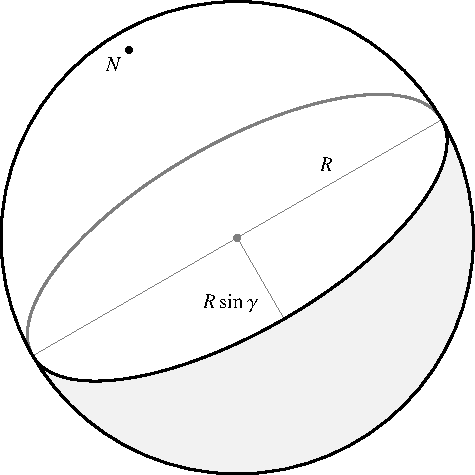
\includegraphics{chapters/5/halb.pdf}
\caption{Aufteilung der sonnenbeschienenen Seite der Erde durch den
Äquator.
\label{skript:halbkugel:teilung}}
\end{figure}%
Die einfachste Erweiterung des Modells von Budyko teilt die
Erde in zwei Halbkugeln auf, die Energie nur langsam austauschen
können.
Für die Energiebilanz brauchen wir daher die Strahlungsleistung
auf einer Halbkugel in Abhängigkeit von der Neigung $\gamma$ der
Erdachse.

Die gesamte auf auf die Erde eingestrahlte Leistung ist $\pi R^2S_0$.
Diese Leistung muss nun in Abhängigkeit von der Neigung $\gamma$
auf die beiden Halbkugeln verteilt werden.
Von der Erde aus gesehen teilt der Äquator die bestrahlte Erde wie
in Abbildung~\ref{skript:halbkugel:teilung} dargestellt.
Der Unterschied zwischen den beiden Halbkugeln ist der Flächeninhalt
der Ellipse, also
\[
F=\pi R^2\sin\gamma.
\]
Die Strahlungsleistung auf den beiden Halbkugeln in
Abbildung~\eqref{skript:halbkugel:teilung} ist daher
\begin{align}
E_N
&= 
\frac12(\pi R^2 S_0 +\pi R^2S_0\sin\gamma)
=
\pi R^2S_0 \frac{1+\sin\gamma}2 = Q\frac{1+\sin\gamma}2
&&\text{Nordhalbkugel,}
\\
E_S
&= 
\frac12(\pi R^2 S_0 -\pi R^2\sin\gamma)
=
\pi R^2S_0 \frac{1-\sin\gamma}2 = Q\frac{1-\sin\gamma}2
&&\text{Südhalbkugel.}
\end{align}
In Kapitel~\ref{chapter:neigung} wird diese Lösung verwendet, um zu
modellieren, wie die Veränderung der Neigung der Erdachse zu Eiszeiten
führen kann.




